
% !TEX TS-program = xelatex
\documentclass[11pt]{article}

\usepackage[a4paper,margin=1in]{geometry}
\usepackage{amsmath,amssymb,mathtools,bm}
\usepackage{physics}
\usepackage{microtype}
\usepackage{hyperref}
\usepackage{caption}
\usepackage{subcaption}
\usepackage{tikz}
\usetikzlibrary{arrows.meta,positioning,calc,decorations.pathmorphing}


\hypersetup{
  colorlinks=true,
  linkcolor=blue,
  citecolor=blue,
  urlcolor=blue
}

\newcommand{\IS}{\mathcal{I}}
\newcommand{\His}{\mathcal{H}_{\mathrm{IS}}}
\newcommand{\Z}{\mathbb{Z}}
\newcommand{\bond}{\langle ij\rangle}

\title{Gauge-Canonical PEPS Ansatz for a Square-Lattice Rydberg Blockade Model\\
{\large Bipartite (A/B) and Directed (L,U in; R,D out) Formulations}}
\author{(technical note)}
\date{\today}

\begin{document}
\maketitle

\begin{abstract}
We document two PEPS parameterizations for a hard Rydberg blockade model on the square lattice
(nearest-neighbor exclusion): (i) a bipartite \emph{A/B} formulation and (ii) a directed-edge formulation
with \emph{incoming} virtual legs $(L,U)$ and \emph{outgoing} legs $(R,D)$.
Both are ``gauge-canonical'' in the sense that the blockade constraint is enforced by fixed, parameter-free
Kronecker-$\delta$ / filter structures, so that forbidden configurations have exactly zero amplitude for
\emph{all} variational parameters. The directed formulation is illustrated with explicit figures.
A short appendix explains the relation to the gauge canonical form (GCF) used for Abelian lattice gauge theory PEPS in
Wu--Liu (2025).
\end{abstract}

\section{Model and constraint}
Consider a square lattice with a two-level Rydberg degree of freedom at each site $i$,
with computational basis $\ket{n_i}$, $n_i\in\{0,1\}$. The hard blockade constraint forbids simultaneous
excitations on nearest neighbors:
\begin{equation}
n_i n_j = 0 \quad \text{for every nearest-neighbor edge } \bond.
\end{equation}
Equivalently, the physical Hilbert space is the \emph{independent-set} subspace
\begin{equation}
\His = \mathrm{span}\{\ket{s}:\; s=\{n_i\}\in\IS\},\qquad
\IS=\{ s:\; n_i n_j=0\ \forall \bond \}.
\end{equation}
In variational Monte Carlo (VMC) one typically samples only $s\in\IS$, and thus never needs to evaluate
wavefunction amplitudes on forbidden configurations. Nevertheless, it is advantageous to build an ansatz
whose amplitude \emph{vanishes exactly} for $s\notin\IS$ at the parameterization level; this removes
redundant degrees of freedom associated with ``nonphysical'' amplitudes.

\section{PEPS notation and virtual-sector decomposition}
A (finite) PEPS defines amplitudes
\begin{equation}
\Psi(s)=\braket{s|\Psi}=
\mathrm{tTr}\Bigl[\ \prod_i \,T^{[i]}_{n_i}\ \Bigr],
\end{equation}
where $T^{[i]}_{n_i}$ is the local tensor at site $i$ with its physical index fixed to $n_i$,
and $\mathrm{tTr}$ denotes contraction of all virtual bonds.

To encode the blockade constraint in a gauge-canonical way, we decompose each virtual bond space into
two \emph{sectors} $k\in\{0,1\}$ (interpreted as ``neighbor not excited'' / ``neighbor excited'')
with a possible degeneracy in each sector. Concretely, each virtual index is taken as
\begin{equation}
a \equiv (k,\mu),\qquad k\in\{0,1\},\qquad \mu=1,\dots,D_k,
\end{equation}
so the total bond dimension is $D=D_0+D_1$. The numbers $D_k$ are the \emph{degeneracies} (or
sector dimensions). The key point is that the blockade logic uses only the sector label $k$, while the
degeneracy indices $\mu$ carry the variational ``entanglement capacity''.

We further define a fixed \emph{filter} function
\begin{equation}
v_k(n)=
\begin{cases}
1, & k=0,\\
1-n, & k=1,
\end{cases}
\qquad n\in\{0,1\}.
\label{eq:vk}
\end{equation}
Thus, if a site is proposed to be excited ($n=1$) while it receives a sector-$1$ message ($k=1$),
then $v_1(1)=0$ kills the amplitude.

\section{Bipartite formulation (A/B)}
\subsection{Lattice bipartition and philosophy}
On a bipartite square lattice, label sublattices as $A$ and $B$ so that every nearest-neighbor bond connects
an $A$ site to a $B$ site.
The A/B formulation implements the blockade as a \emph{copy--filter} mechanism:
\begin{itemize}
\item On an $A$ site, the tensor \emph{copies} its occupation $n$ into the sector label $k$ on all adjacent bonds.
\item On a $B$ site, the tensor \emph{filters}: if it is excited ($n=1$), it requires that all neighbor sectors are $k=0$.
\end{itemize}
The resulting ansatz has exactly zero amplitude whenever an adjacent pair of excitations appears.

\begin{figure}[t]
\centering
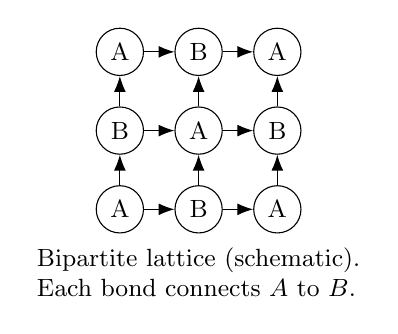
\begin{tikzpicture}[scale=1.0, every node/.style={font=\small}]
  % draw a 3x3 patch with bipartite coloring
  \foreach \x in {0,1,2}{
    \foreach \y in {0,1,2}{
      \pgfmathparse{mod(\x+\y,2)==0 ? "A" : "B"}
      \let\lab\pgfmathresult
      \node[draw, circle, minimum size=6mm, inner sep=0pt] (n\x\y) at (\x,\y) {\lab};
    }
  }
  % bonds
  \foreach \x/\y/\xx/\yy in {0/0/1/0,1/0/2/0,0/1/1/1,1/1/2/1,0/2/1/2,1/2/2/2,
                            0/0/0/1,0/1/0/2,1/0/1/1,1/1/1/2,2/0/2/1,2/1/2/2}{
    \draw[-{Latex[length=2mm]}] (n\x\y) -- (n\xx\yy);
  }
  \node[align=left] at (1,-0.8) {Bipartite lattice (schematic).\\Each bond connects $A$ to $B$.};
\end{tikzpicture}
\caption{Schematic A/B bipartition used in the bipartite formulation. The arrows are only illustrative (one may treat the bonds as undirected); the essential ingredient is that every bond connects an $A$ site to a $B$ site.}
\label{fig:bipartite}
\end{figure}

\subsection{A-sublattice tensor: copy to sectors}
Let the four virtual legs be labeled $(L,R,U,D)$ and each index be $a_e=(k_e,\mu_e)$.
On an $A$ site we define
\begin{equation}
T^{[A]}_{\,n;\,(k_L,\mu_L)(k_R,\mu_R)(k_U,\mu_U)(k_D,\mu_D)}
=
\Bigl[\prod_{e\in\{L,R,U,D\}}\delta_{k_e,n}\Bigr]\;
A^{[A]}_{\,n;\,\mu_L\mu_R\mu_U\mu_D},
\label{eq:A_copy}
\end{equation}
where the core tensors $A^{[A]}_{n}$ are variational parameters. Equation~\eqref{eq:A_copy} enforces
that all adjacent bond sectors equal the physical occupation $n$ on $A$.

\subsection{B-sublattice tensor: filter}
On a $B$ site we impose a filtering structure. A convenient (general) canonical choice is
\begin{equation}
T^{[B]}_{\,n;\,(k_L,\mu_L)(k_R,\mu_R)(k_U,\mu_U)(k_D,\mu_D)}
=
\Bigl[\prod_{e\in\{L,R,U,D\}} v_{k_e}(n)\Bigr]\;
B^{[B]}_{\,n;\,k_Lk_Rk_Uk_D;\,\mu_L\mu_R\mu_U\mu_D}.
\label{eq:B_filter}
\end{equation}
Because $v_1(1)=0$, if the $B$ site is excited ($n=1$), then every adjacent sector must satisfy $k_e=0$.
The tensor blocks $B^{[B]}_{n;\,k_Lk_Rk_Uk_D}$ are the variational parameters, but they are only sampled
in the sector combinations compatible with the physical configuration.

\subsection{Exact blockade}
Consider a nearest-neighbor bond connecting an $A$ site $i$ to a $B$ site $j$.
From the $A$ tensor, the shared sector on that bond is fixed to $k=n_i$ by the $\delta$ constraint.
If both sites were excited ($n_i=n_j=1$), then the $B$ tensor contributes a factor $v_{k}(n_j)=v_{1}(1)=0$,
hence $\Psi(s)=0$. Therefore the amplitude vanishes identically for any configuration containing an adjacent
pair of excitations.

\section{Directed formulation: $(L,U)$ incoming, $(R,D)$ outgoing}
\subsection{Directed-edge convention}
Fix a \emph{global} orientation of the square lattice bonds so that at every site:
\begin{itemize}
\item the \textbf{incoming} virtual legs are \emph{Left} $(L)$ and \emph{Up} $(U)$;
\item the \textbf{outgoing} virtual legs are \emph{Right} $(R)$ and \emph{Down} $(D)$.
\end{itemize}
Equivalently, every horizontal bond is oriented left$\to$right, and every vertical bond is oriented top$\to$bottom.
This choice makes every site both a receiver (from $L,U$) and a sender (to $R,D$), while keeping a single,
translation-invariant tensor type.

\begin{figure}[t]
\centering
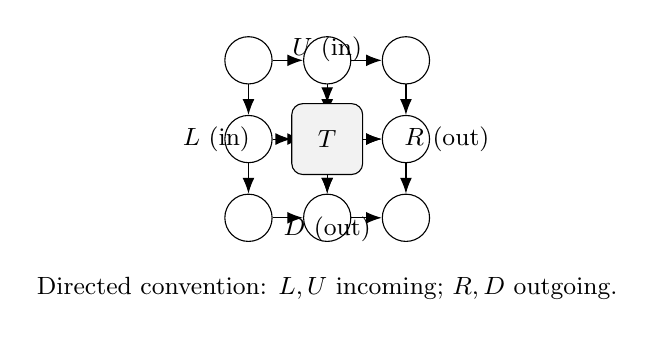
\begin{tikzpicture}[scale=1.0, every node/.style={font=\small}]
  % 3x3 nodes
  \foreach \x in {0,1,2}{
    \foreach \y in {0,1,2}{
      \node[draw, circle, minimum size=6mm, inner sep=0pt] (n\x\y) at (\x,\y) {};
    }
  }
  % horizontal arrows: left to right
  \foreach \y in {0,1,2}{
    \foreach \x in {0,1}{
      \draw[-{Latex[length=2mm]}] (n\x\y) -- (n\the\numexpr\x+1\relax\y);
    }
  }
  % vertical arrows: top to bottom
  \foreach \x in {0,1,2}{
    \foreach \y in {1,2}{
      \draw[-{Latex[length=2mm]}] (n\x\y) -- (n\x\the\numexpr\y-1\relax);
    }
  }

  % highlight central site
  \node[draw, rectangle, rounded corners, minimum width=9mm, minimum height=9mm, fill=gray!10] (c) at (1,1) {$T$};
  \node[above=4mm of c] (labU) {$U$ (in)};
  \node[left=4mm of c] (labL) {$L$ (in)};
  \node[right=4mm of c] (labR) {$R$ (out)};
  \node[below=4mm of c] (labD) {$D$ (out)};

  \draw[-{Latex[length=2mm]}] (n01) -- (c.west);
  \draw[-{Latex[length=2mm]}] (n12) -- (c.north);
  \draw[-{Latex[length=2mm]}] (c.east) -- (n21);
  \draw[-{Latex[length=2mm]}] (c.south) -- (n10);

  \node[align=left] at (1,-0.9) {Directed convention: $L,U$ incoming; $R,D$ outgoing.};
\end{tikzpicture}
\caption{Directed-edge convention for the translation-invariant formulation: all horizontal bonds are oriented left$\to$right and all vertical bonds top$\to$bottom. For the highlighted tensor $T$, legs $(L,U)$ are incoming and $(R,D)$ are outgoing.}
\label{fig:directed_convention}
\end{figure}

\subsection{Local tensor definition (gauge-canonical form)}
Each virtual leg carries an index $a=(k,\mu)$ with $k\in\{0,1\}$ and $\mu=1,\dots,D_k$.
Define a single site tensor (valid for all sites) as
\begin{align}
&T_{\,n;\,(k_L,\mu_L)(k_U,\mu_U)(k_R,\mu_R)(k_D,\mu_D)}
\notag\\
&\qquad =
\underbrace{\delta_{k_R,n}\,\delta_{k_D,n}}_{\text{copy to outgoing sectors}}
\ \underbrace{v_{k_L}(n)\,v_{k_U}(n)}_{\text{filter incoming sectors}}
\ \times\
C^{(k_L,k_U)}_{\,n;\,\mu_L\mu_U\mu_R\mu_D}.
\label{eq:direct_T}
\end{align}
Here $C^{(k_L,k_U)}_{n}$ is the variational \emph{core tensor} (degeneracy part), while all
$\delta$ and $v_k$ factors are fixed and parameter-free.

\begin{figure}[t]
\centering
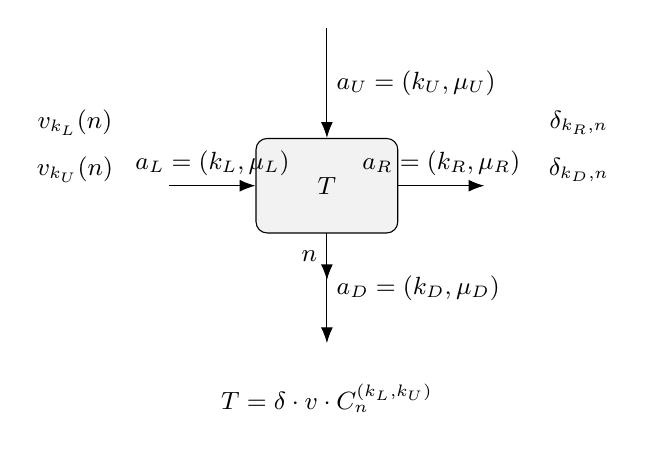
\begin{tikzpicture}[scale=1.0, every node/.style={font=\small}]
  \node[draw, rectangle, rounded corners, minimum width=18mm, minimum height=12mm, fill=gray!10] (T) at (0,0) {$T$};

  % legs
  \draw[-{Latex[length=2mm]}] (-2,0) -- (T.west) node[midway,above] {$a_L=(k_L,\mu_L)$};
  \draw[-{Latex[length=2mm]}] (0,2) -- (T.north) node[midway,right] {$a_U=(k_U,\mu_U)$};
  \draw[-{Latex[length=2mm]}] (T.east) -- (2,0) node[midway,above] {$a_R=(k_R,\mu_R)$};
  \draw[-{Latex[length=2mm]}] (T.south) -- (0,-2) node[midway,right] {$a_D=(k_D,\mu_D)$};

  % physical leg
  \draw[-{Latex[length=2mm]}] (0, -0.6) -- (0,-1.2) node[midway,left] {$n$};

  % annotations
  \node[align=left] at (3.2,0.8) {$\delta_{k_R,n}$};
  \node[align=left] at (3.2,0.2) {$\delta_{k_D,n}$};
  \node[align=left] at (-3.2,0.8) {$v_{k_L}(n)$};
  \node[align=left] at (-3.2,0.2) {$v_{k_U}(n)$};

  \node[align=left] at (0,-2.7) {$T=\delta\cdot v\cdot C^{(k_L,k_U)}_n$};
\end{tikzpicture}
\caption{Structure of the directed-formulation site tensor \eqref{eq:direct_T}. Outgoing sectors $(R,D)$ are fixed to the physical occupation by Kronecker deltas, while incoming sectors $(L,U)$ are filtered by $v_k(n)$ with $v_1(1)=0$. The degeneracy indices $\mu$ carry the variational core tensor $C^{(k_L,k_U)}_n$.}
\label{fig:directed_tensor}
\end{figure}

\subsection{Block structure}
Equation~\eqref{eq:direct_T} implies a sparse block structure:
\begin{itemize}
\item If $n=1$, the filter factors enforce $k_L=k_U=0$ (since $v_1(1)=0$), while the deltas enforce
$k_R=k_D=1$. Thus there is a \emph{single} nonzero sector pattern:
\begin{equation}
(n=1):\quad (k_L,k_U,k_R,k_D)=(0,0,1,1),
\end{equation}
with core block shape $D_0\times D_0\times D_1\times D_1$ (for $\mu_L,\mu_U,\mu_R,\mu_D$).
\item If $n=0$, the deltas enforce $(k_R,k_D)=(0,0)$, while $(k_L,k_U)\in\{0,1\}^2$ are allowed.
So there are four $n=0$ blocks labelled by $(k_L,k_U)$, with shapes
$D_{k_L}\times D_{k_U}\times D_0\times D_0$.
\end{itemize}
The key algorithmic property is that, for any fixed physical configuration $s$, the sector labels $k$
on every bond are uniquely fixed by the source site (because of the outgoing deltas).
Hence the single-layer network $\braket{s|\Psi}$ contracts only the corresponding degeneracy dimensions.

\subsection{Exact blockade: local two-site argument}
Consider a directed bond $i\to j$ (either horizontal or vertical).
By the outgoing constraints at $i$, the bond sector equals the occupation:
\begin{equation}
k_{i\to j}=n_i.
\end{equation}
At site $j$ this sector enters as an incoming leg (either $L$ or $U$), contributing a factor
$v_{k_{i\to j}}(n_j)$. If both sites are excited ($n_i=n_j=1$), then $k_{i\to j}=1$ and
\begin{equation}
v_{k_{i\to j}}(n_j)=v_{1}(1)=0,
\end{equation}
so the amplitude vanishes. Therefore $\Psi(s)=0$ for any configuration containing an adjacent $11$,
independently of the variational core tensor $C$.

\begin{figure}[t]
\centering
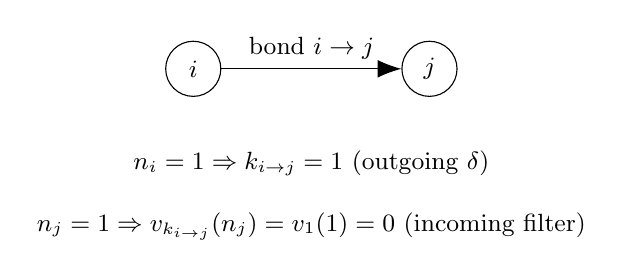
\begin{tikzpicture}[scale=1.0, every node/.style={font=\small}]
  \node[draw, circle, minimum size=7mm] (i) at (0,0) {$i$};
  \node[draw, circle, minimum size=7mm] (j) at (3,0) {$j$};
  \draw[-{Latex[length=3mm]}] (i) -- (j) node[midway,above] {bond $i\to j$};

  \node[align=left] at (1.5,-1.2) {$n_i=1 \Rightarrow k_{i\to j}=1$ (outgoing $\delta$)};
  \node[align=left] at (1.5,-2.0) {$n_j=1 \Rightarrow v_{k_{i\to j}}(n_j)=v_1(1)=0$ (incoming filter)};
\end{tikzpicture}
\caption{Two-site mechanism enforcing the blockade in the directed formulation. If $i$ is excited, the outgoing delta fixes the bond sector to $k=1$. If $j$ is also excited, the incoming filter produces $v_1(1)=0$, killing the amplitude.}
\label{fig:two_site_blockade}
\end{figure}

\section{Remarks on redundancy and SR stability}
The constructions above remove redundancy associated with amplitudes of forbidden configurations:
those amplitudes are identically zero at the ansatz level, so there are no parameters whose only role
would be to tune nonphysical weights.

A separate and unavoidable issue is the intrinsic \emph{PEPS gauge redundancy} on internal virtual bonds:
inserting $X$ and $X^{-1}$ on a bond leaves the physical state invariant. In stochastic reconfiguration (SR)
or time-dependent VMC (tVMC), the infinitesimal generators of these gauge transformations appear as null
vectors of the log-derivative matrix and the quantum geometric tensor. Analytic gauge removal procedures
(e.g.\ QR projection or minSR formulations) can be used to stabilize the SR equation.

\appendix
\section{Relation to the gauge canonical form for lattice gauge theory PEPS (minimal)}
Wu and Liu (2025) formulate gauge-invariant PEPS for Abelian lattice gauge theories by assigning a conserved
\emph{charge} to each virtual index and enforcing a local Gauss-law constraint as a block-sparsity condition.
In their notation, the bond dimension decomposes as
\begin{equation}
D=\sum_{k} D_k,
\end{equation}
where $D_k$ is the \emph{degeneracy} (multiplicity) of charge sector $k$ (the number of virtual basis states carrying charge $k$).
They further identify a \emph{gauge canonical form} (GCF) in which the link (gauge) tensor becomes parameter-free:
\begin{equation}
B^{n}_{lr}=\delta_{lr}\,\delta_{n,q(l)}\,\delta_{n,q(r)},
\end{equation}
so only the matter tensors remain variational. In VMC, each sampled physical configuration uniquely selects the
charge sector on each bond; consequently, the effective bond dimension of the single-layer network reduces from the
total $D$ to the relevant $D_k$ on that bond, providing a substantial computational simplification.

The Rydberg-blockade PEPS constructions above are a direct analogue of this logic. The sector label $k\in\{0,1\}$
plays the role of the ``charge'' (or electric-field value) carried by a virtual index. The fixed delta / filter structures
in Eqs.~\eqref{eq:A_copy}--\eqref{eq:direct_T} are the blockade counterpart of the parameter-free GCF link tensor:
they enforce the hard constraint and remove variational parameters from the constraint part of the ansatz.
The remaining degeneracy indices $\mu$ correspond to the degeneracy dimensions $D_k$ in the gauge-theory setting.
Finally, because outgoing deltas (or the bipartite copy tensor) fix sector values bond-by-bond, every sampled independent-set
configuration selects a unique sector pattern, so that the single-layer contraction only involves the corresponding $D_k$
channels, exactly mirroring the ``configuration selects sector'' feature emphasized in the lattice gauge theory PEPS literature.

\vspace{1em}
\noindent\textbf{Reference.} Y. Wu and W.-Y. Liu, \emph{Accurate Gauge-Invariant Tensor-Network Simulations for Abelian Lattice Gauge Theory in (2+1)D: Ground-State and Real-Time Dynamics}, Phys.\ Rev.\ Lett.\ \textbf{135}, 130401 (2025).
\end{document}